\section{BEVFormer v2}
将现代2D图像骨干网络（Image Backbone）适配到BEV识别中，无需繁琐的深度预训练（Depth Pre-training），将为下游自动驾驶任务开启许多可能性。
本文提出 BEVFormer v2，一种两阶段（Two-stage）BEV检测器，同时结合BEV和透视监督（Perspective Supervision），在BEV检测中无障碍地采用图像骨干网络。

\subsection{整体架构}
如图 \ref{fig:architecture} 所示，BEVFormer v2 主要由五个组件构成：图像骨干网络、透视3D检测头（Perspective 3D Detection Head）、空间编码器（Spatial Encoder）、改进的时序编码器（Temporal Encoder）和BEV检测头（BEV Detection Head）。
与原始 BEVFormer~\cite{bevformer} 相比，除空间编码器外所有组件均进行了修改。
具体而言，BEVFormer v2 使用的所有图像骨干网络均未使用任何自动驾驶数据集或深度估计数据集进行预训练。
引入透视3D检测头以促进2D图像骨干网络的适配，并为BEV检测头生成物体提议（Object Proposal）。
采用新的时序BEV编码器以更好地整合长期时序信息。
BEV检测头现在接收混合物体查询（Hybrid Object Query）集作为输入。本文将第一阶段提议与可学习物体查询结合，形成新的混合物体查询用于第二阶段。

\subsection{透视监督}
本文首先分析鸟瞰视图模型的问题，以解释为何需要额外的监督。
典型的BEV模型维护附着在BEV平面上的网格状特征，其中每个网格从多视角图像对应2D像素的特征中聚合3D信息。
模型基于BEV特征预测目标物体的3D边界框，本文将这种施加在BEV特征上的监督称为BEV监督（BEV Supervision）。
以 BEVFormer \cite{bevformer} 为例，其使用编码器-解码器结构生成和利用BEV特征。
编码器为BEV平面上的每个网格单元分配一组3D参考点（Reference Point），并将它们投影到多视角图像上作为2D参考点。
然后，在2D参考点周围采样图像特征，利用空间交叉注意力（Spatial Cross-attention）将其聚合为BEV特征。
解码器是一个可变形 DETR（Deformable DETR）\cite{deformable-detr} 头，使用少量固定数量的物体查询（Object Query）在BEV坐标系中预测3D边界框。
图 \ref{fig:supervision} 展示了由3D到2D视图变换和 DETR \cite{DETR} 头引入的BEV监督的两个潜在问题：
\begin{itemize}
    \item 监督对于图像特征是隐式的（Implicit）。损失直接作用于BEV特征，经过3D到2D的投影和图像特征的注意力采样后变为间接。
    \item 监督对于图像特征是稀疏的（Sparse）。只有少量被物体查询关注的BEV网格对损失有贡献，因此仅有这些网格的2D参考点周围的稀疏像素获得监督信号。
\end{itemize}
因此，训练中出现不一致性：BEV检测头依赖于图像特征中包含的3D信息，但骨干网络如何编码这些信息却缺少足够的指导。

\label{sec:perspective_supervision}
\begin{figure}[t]
    \centering
    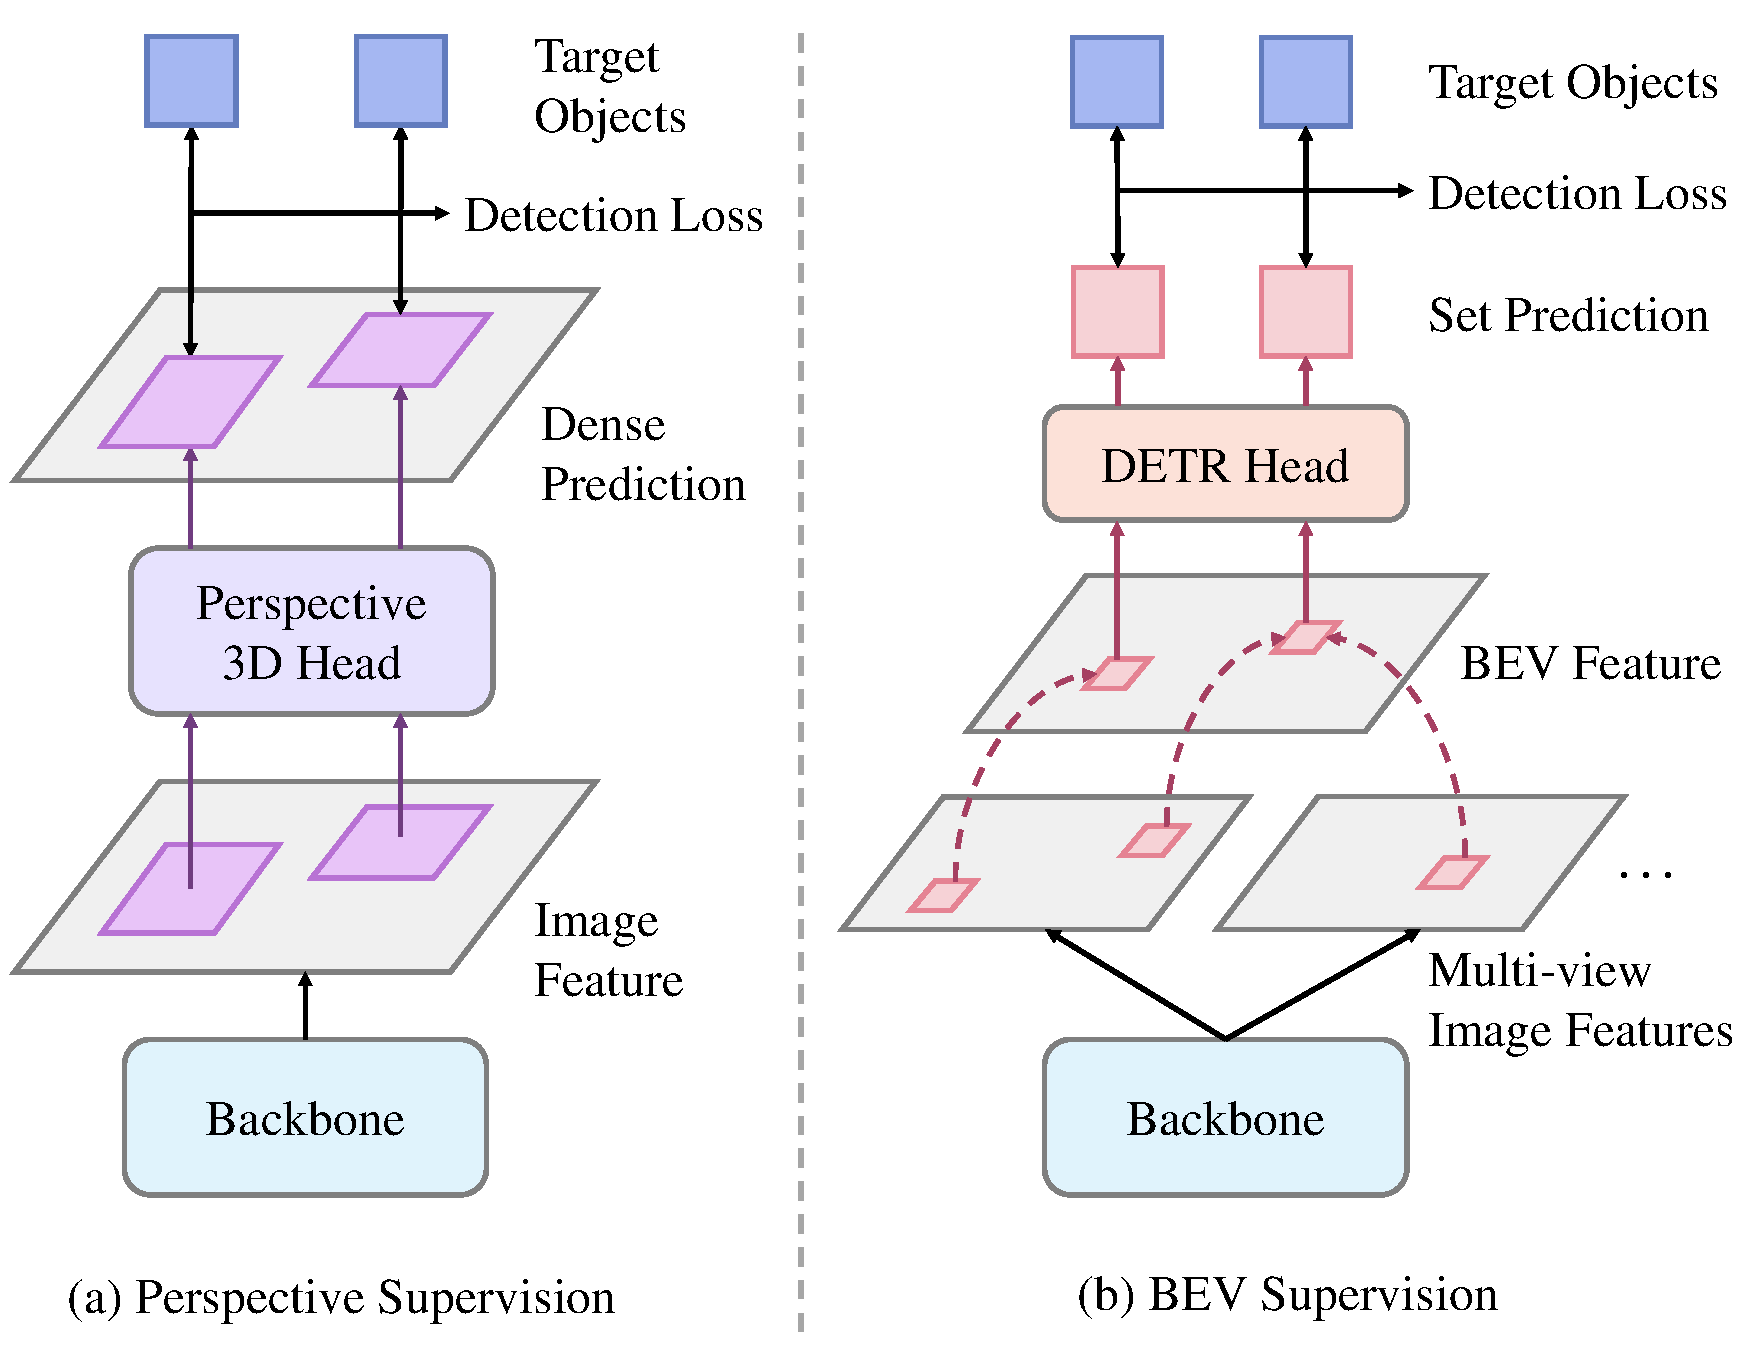
\includegraphics[width=1.0\linewidth]{figures/supervision.pdf}
    \caption{透视监督（a）与 BEV 监督（b）的对比。透视检测器的监督信号对图像特征是密集且直接的，而BEV检测器的监督信号则是稀疏且间接的。}
    \label{fig:supervision}
\end{figure}

先前的BEV方法并未严重受到此不一致性的影响，甚至可能未意识到该问题。
这是因为其骨干网络要么规模较小，要么已在带有单目检测头的3D检测任务上进行了预训练。
与BEV头相反，透视3D头在图像特征上进行逐像素预测，为适配2D图像骨干网络提供了更丰富的监督信号。
本文将施加在图像特征上的监督定义为透视监督。
如图 \ref{fig:supervision} 所示，与BEV监督不同，透视检测损失直接且密集地作用于图像特征。
本文认为透视监督显式地指导骨干网络感知3D场景并提取有用信息（例如物体的深度和朝向），克服了BEV监督的缺陷，因此在使用现代图像骨干网络训练BEV模型时至关重要。

\subsection{透视损失}
根据前述分析，透视监督是优化BEV模型的关键。
在 BEVFormer v2 中，本文通过辅助透视损失（Auxiliary Perspective Loss）引入透视监督。
具体而言，在骨干网络上构建一个透视3D检测头，用于在透视图上检测目标物体。
本文采用类似 FCOS3D~\cite{fcos3d} 的检测头，预测3D边界框的中心位置、尺寸、朝向和投影中心度（Projected Center-ness）。
该检测头的检测损失（称为透视损失 $\mathcal{L}_{pers}$）作为BEV损失 $\mathcal{L}_{bev}$ 的补充，促进骨干网络的优化。
整个模型的总目标函数为：
\begin{equation}
\mathcal{L}_{total} = \lambda_{bev}\mathcal{L}_{bev}+\lambda_{pers}\mathcal{L}_{pers}.
\end{equation}

\subsection{改进的时序编码器}
BEVFormer 使用循环时序自注意力（Recurrent Temporal Self-attention）来整合历史BEV特征。
但该时序编码器在利用长期时序信息方面存在不足，简单地将循环步数从4增加到16并不能带来额外的性能提升。

本文为 BEVFormer v2 重新设计了时序编码器，采用简单的扭曲拼接（Warp and Concatenate）策略。
给定不同帧 $k$ 的BEV特征 $B_k$，首先根据帧 $t$ 和帧 $k$ 之间的参考帧变换矩阵 $T_k^{t} = [\bf{R} | \bf{t}] \in \text{SE3}$，将 $B_k$ 双线性扭曲到当前帧得到 $B_k^t$。
然后沿通道维度拼接历史BEV特征与当前BEV特征，并使用残差块（Residual Block）进行降维。
为保持与原始设计相似的计算复杂度，本文使用相同数量的历史BEV特征但增加了采样间隔。
除了利用长期时序信息外，新的时序编码器还开启了在离线3D检测设置中利用未来BEV特征的可能性。

\subsection{两阶段BEV检测器}
尽管两个检测头的联合训练已经提供了足够的监督，但本文从不同视图各自获得两组检测结果。
本文并未采用直接使用BEV头的预测并丢弃透视图头的预测，或通过NMS启发式地合并两组预测的做法，而是设计了一种将两个头整合为两阶段预测流程的新颖结构，即两阶段BEV检测器。
BEV头中的物体解码器（Object Decoder）是一个 DETR \cite{DETR} 解码器，使用一组可学习的嵌入（Learned Embedding）作为物体查询，通过训练学习目标物体可能的位置。
然而，随机初始化的嵌入需要很长时间来学习合适的位置。
此外，学习到的物体查询在推理时对所有图像固定不变，由于物体的空间分布可能变化，这可能不够精准。
为解决这些问题，透视图头的预测经过后处理筛选后融合到解码器的物体查询中，形成两阶段流程。
这些混合物体查询提供了高分（高概率）的候选位置，使BEV头在第二阶段更容易捕捉目标物体。混合物体查询解码器的细节将在后文描述。
需要注意的是，第一阶段提议不一定来自透视检测器——例如可以来自另一个BEV检测器——但实验表明，只有来自透视图的预测对第二阶段BEV头有帮助。

\subsection{混合物体查询解码器}
为了将第一阶段提议融合到第二阶段的物体查询中，BEVFormer v2 中BEV头的解码器在 BEVFormer \cite{bevformer} 使用的可变形 DETR（Deformable DETR）\cite{deformable-detr} 解码器基础上进行了修改。
解码器由堆叠的交替自注意力（Self-attention）和交叉注意力（Cross-attention）层组成。
交叉注意力层是一个可变形注意力模块 \cite{deformable-detr}，接收以下三个元素作为输入：
(1) 内容查询（Content Query）——用于生成采样偏移和注意力权重的查询特征。
(2) 参考点（Reference Point）——值特征上的2D点，作为每个查询的采样参考。
(3) 值特征（Value Feature）——被关注的BEV特征。
在原始 BEVFormer \cite{bevformer} 中，内容查询是一组可学习的嵌入，参考点通过线性层从一组可学习的位置嵌入预测得到。
在 BEVFormer v2 中，本文从透视头获取提议，并通过后处理筛选部分提议。
%as described in ~\cref{sec/appendix/post-process}.
如图 \ref{fig:decoder} 所示，被选提议在BEV平面上投影的框中心用作逐图像参考点，并与从位置嵌入生成的逐数据集参考点相结合。
逐图像参考点直接指示物体在BEV平面上可能存在的位置，使解码器更容易检测目标物体。
然而，由于遮挡或出现在相邻视图边界，少量物体可能未被透视头检测到。
为避免遗漏这些物体，本文保留原始逐数据集参考点，通过学习空间先验来捕获它们。

\begin{figure}[t]
    \centering
    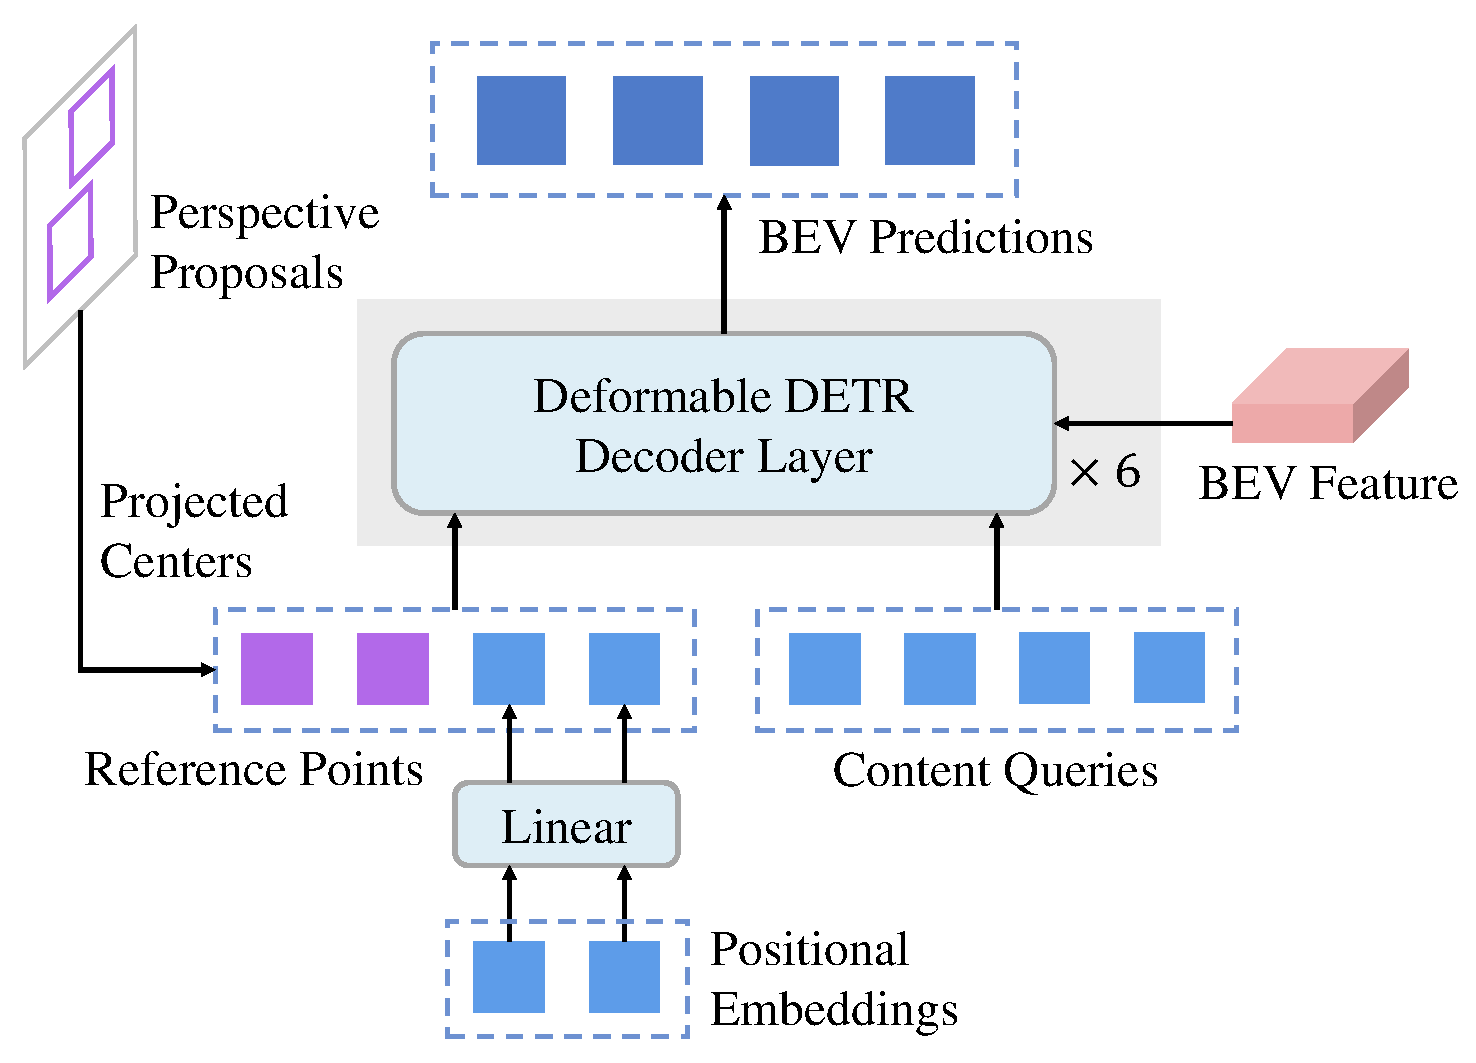
\includegraphics[width=1.0\linewidth]{figures/decoder.pdf}
    \caption{BEVFormer v2 中 BEV 头的解码器。第一阶段提议的投影中心用作逐图像参考点（紫色），与逐数据集学习的内容查询和位置嵌入（蓝色）结合为混合物体查询。}
    \label{fig:decoder}
    \vspace{-0.3cm}
\end{figure}
